%----------------------------------------------------------------------------
\chapter{\projectoverview}
%----------------------------------------------------------------------------
\section{A vállalat és az üzleti igények}

A projekt célja a \textbf{TéDé Rendezvények} vállalat bérlés és projektkezelési folyamatainak teljes digitalizálása volt. 
A korábbi papíralapú és Excel-alapú folyamatok nem feleltek meg a vállalat növekvő igényeinek,
és egy modern, integrált rendszer kialakítása vált szükségessé. Az online elérhető üzenetküldő és felhő alapú megoldások
nem kínáltak megfelelő rugalmasságot és testreszabhatóságot, ezért egy egyedi fejlesztésű rendszer mellett született döntés.

\textbf{A vállalat számára kiemelten fontos volt egy egységes, modern és felhasználóbarát rendszer, amely:}
\begin{itemize}
    \item automatizálja a bérlési folyamatokat,
    \item nyomon követi a készleteket,
    \item biztosítja az adminisztráció teljes körű kezelését,
    \item egyszerűsíti a munkafolyamatokat,
    \item csökkenti a hibalehetőségeket,
    \item javítja a kommunikációt a csapaton belül,
    \item egységesíti a dokumentációt,
    \item minden információ egy helyen elérhető,
    \item lehetővé teszi a gyors árajánlatkészítést.
\end{itemize}

\pagebreak
\textbf{További célok voltak:}
\begin{itemize}
    \item modern, felhasználóbarát felület
    \item egyszerűen telepíthető és skálázható \textbf{Docker} segítségével
    \item könnyen karbantartható és bővíthető architektúra
    \item biztonságos hozzáférés-kezelés és jogosultságok
    \item részletes riportálási és statisztikai funkciók
\end{itemize}

%----------------------------------------------------------------------------
\section{A projekt összetettsége és kihívásai}
%----------------------------------------------------------------------------

A projekt felettébb összetettnek tekinthető, mivel:
\begin{itemize}
    \item többféle felhasználói szerepkört kellett kezelnie (admin, munkatárs, menedzser),
    \item integrálni kellett különböző adatforrásokat és a bérlési folyamatokat,
    \item biztonsági és hozzáférés-kezelési követelményeknek kellett megfelelnie,
    \item a fejlesztés során több technológiát kellett összehangolni a rugalmasság és megbízhatóság érdekében.
\end{itemize}

%----------------------------------------------------------------------------
\section{Technológiai háttér}
%----------------------------------------------------------------------------

A rendszer fejlesztése a következő technológiákra épült:
\begin{itemize}
    \item \textbf{Backend:} PHP a Twig sablonmotorral,
    \item \textbf{Frontend:} modern responsive felhasználói felület Twig sablonokkal,
    \item \textbf{Konténerizálás és telepítés:} Docker és Docker Compose, előre elkészített konténerekben,
    \item \textbf{Konfiguráció:} testreszabható \texttt{.env} fájlok segítségével.
    \item \textbf{Reverse proxy:} Nginx a kérések kezelésére és a statikus fájlok kiszolgálására,
    \item \textbf{Adatbázis:} MySQL a megbízható adatkezelés érdekében,
    \item \textbf{Verziókezelés:} Git a kód nyomon követésére.
\end{itemize}

%----------------------------------------------------------------------------
\section{A megvalósított szoftver}
%----------------------------------------------------------------------------
\subsection{Bejelentkezés}
%----------------------------------------------------------------------------
A Bejelentkezési felület lehetővé teszi a felhasználók számára, hogy biztonságosan hozzáférjenek a rendszerhez.
Ezt megtehetik helyi fiókkal vagy Google OAuth2 hitelesítéssel, amely egyszerűsíti a bejelentkezési folyamatot és növeli a biztonságot.
A bejelentkezés után amennyiben új felhasználó lép be a rendszerbe, egy egyszeri csatlkozó jelszó megadására van szükség amivel kapcsolódik a vállalathoz,
ezzel biztosítva, hogy csak jogosult személyek férjenek hozzá a rendszerhez, és minden tevékenység naplózásra kerül a későbbi ellenőrzés érdekében.
%----------------------------------------------------------------------------
\begin{figure}[H]
	\centering
    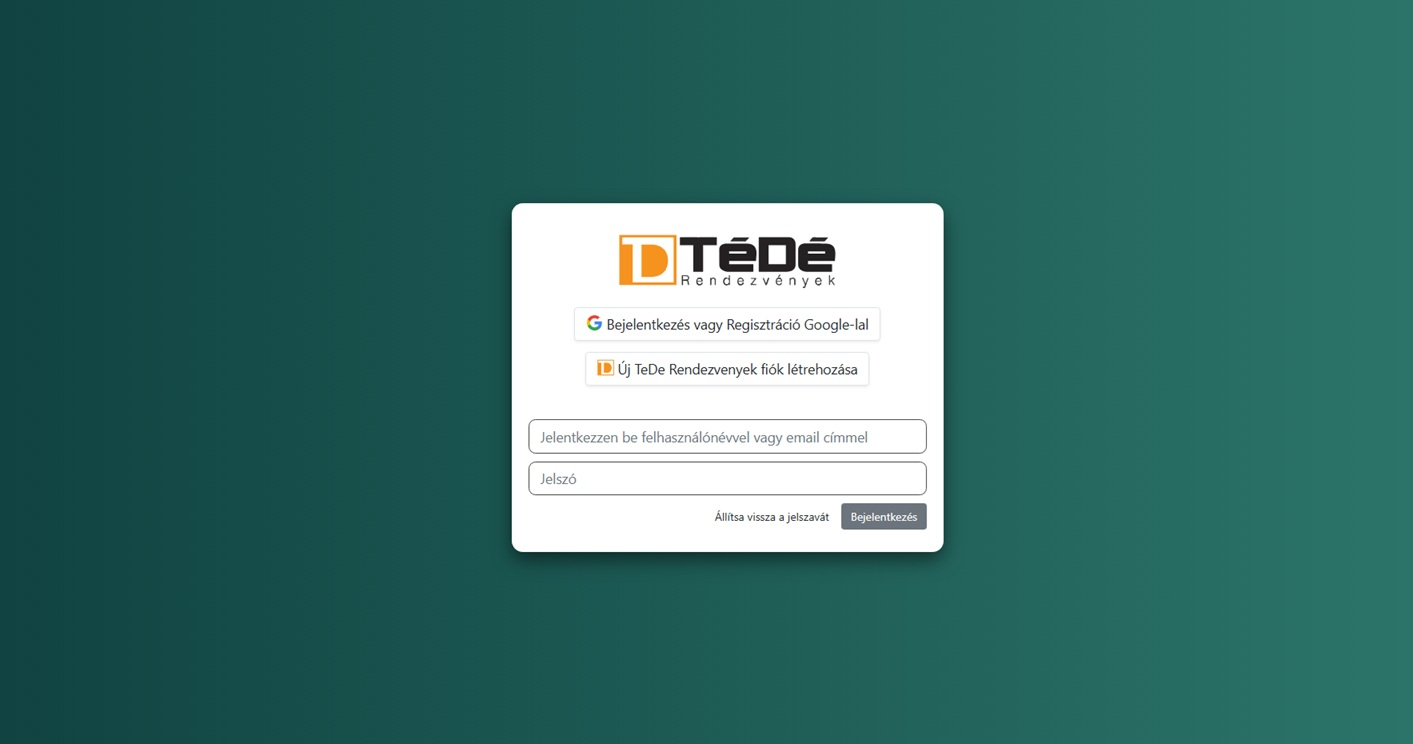
\includegraphics[width=150mm, keepaspectratio]{figures/login.jpg}
    \caption{Bejelentkezés}
    \label{fig:login}
\end{figure}
%----------------------------------------------------------------------------
\subsection{Dashboard}
%----------------------------------------------------------------------------

Az alkalmazás indítása után az alapértelmezett nézet a \textbf{Dashboard}, amely a rendszer központi irányítópultjaként szolgál.  
Célja, hogy a felhasználó egyetlen felületen, átlátható formában kapjon átfogó képet a vállalkozás aktuális működéséről, 
az eszközállományról, a projektek státuszáról és a saját napi tevékenységeiről.

A felület moduláris felépítésű, azaz minden információ önálló panelen jelenik meg, 
így a felhasználó gyorsan hozzáférhet az őt érdeklő adatokhoz anélkül, hogy menük között kellene navigálnia.  
A legfontosabb panelek a következők:

\begin{itemize}
    \item \textbf{Eszköz statisztika:} összesített információkat jelenít meg az aktuális eszközpark állapotáról, 
    beleértve az összértéket, az össztömeget, a raktárban lévő mennyiséget és az eszköztípusok számát.  
    Ez különösen hasznos a logisztikai és bérléskezelési döntések előkészítésénél.
    
    \item \textbf{Tároló használat:} kijelzi a tárhely aktuális kihasználtságát, ami segíti a rendszeradminisztrátort a 
    tárolókapacitás hatékony felügyeletében, különösen a feltöltött képek és dokumentumok kezelésénél.
    
    \item \textbf{Felhasználók:} megjeleníti az aktív felhasználók számát, ezzel is elősegítve a jogosultságkezelést és a hozzáférések ellenőrzését.
    
    \item \textbf{Projekt statisztika:} az éppen aktív és a lezárt projektek számát mutatja, 
    ami egyértelmű képet ad a vállalat aktuális munkaterheléséről és projektfázisairól.
    
    \item \textbf{Karbantartási feladatok:} listázza a függő karbantartási műveleteket, illetve a bejelentkezett felhasználó saját feladatait, 
    ezzel biztosítva, hogy a rendszerüzemeltetés és az eszközkarbantartás ne maradjon el.
\end{itemize}

A jobb oldalon található \textbf{naptárnézet} a Dashboard egyik kulcsfunkciója, amely a tervezés és szervezés hatékonyságát támogatja.  
A naptár kétféle módon használható:

\begin{itemize}
    \item \textbf{Vállalati nézet:} az összes eseményt, projektmérföldkövet és karbantartási ütemezést megjeleníti, így a vezetők és adminisztrátorok 
    teljes képet kapnak a szervezet aktuális feladatairól.
    \item \textbf{Személyes nézet:} kizárólag az adott felhasználóhoz rendelt eseményeket és határidőket mutatja, 
    ezzel segítve az egyéni időbeosztás és feladatprioritás kezelését.
\end{itemize}

A naptár interaktív: a felhasználók közvetlenül a felületen lépkedhetnek a hetek és hónapok között, 
illetve eseményekhez kapcsolódó részleteket is megtekinthetnek.  
Ez a funkció jelentősen növeli a munkaszervezés hatékonyságát, mivel vizuális formában támogatja a tervezést és a határidők követését.

A Dashboard tehát nem csupán egy információs felület, hanem a rendszer működésének központi irányítási pontja, 
amely valós időben tükrözi a vállalkozás operatív állapotát.  
Felépítése reszponzív, így asztali és mobil eszközön egyaránt optimálisan használható, 
miközben a modulok dinamikusan frissülnek a háttérben futó adatbázis-lekérdezések alapján.

%----------------------------------------------------------------------------
\begin{figure}[H]
	\centering
    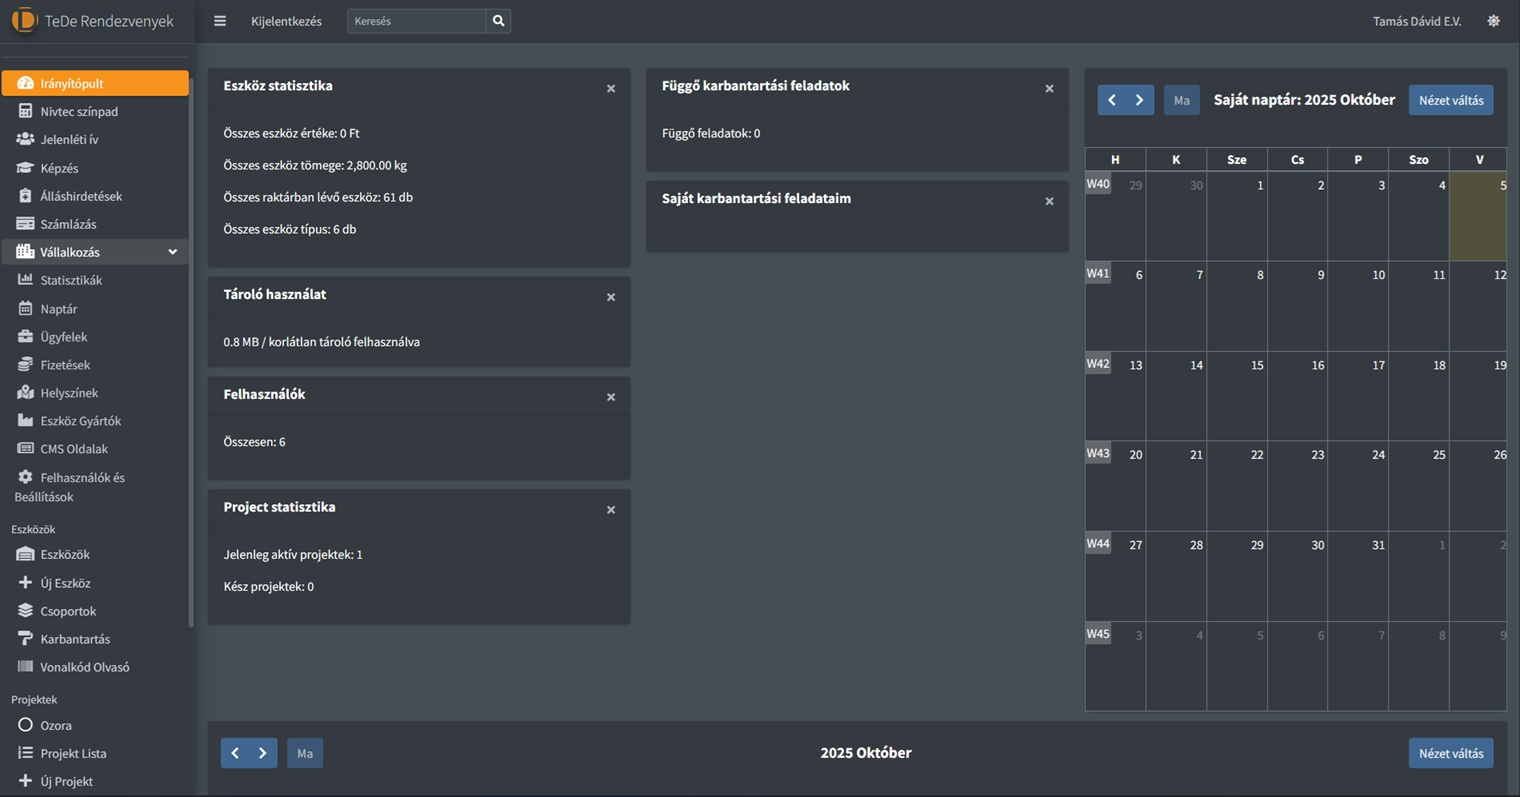
\includegraphics[width=150mm, keepaspectratio]{figures/dashboard.jpg}
    \caption{Dashboard – vállalati áttekintő felület}
    \label{fig:dashboard}
\end{figure}
%----------------------------------------------------------------------------

\subsection{Eszközök kezelése}
%----------------------------------------------------------------------------

Az \textbf{Eszközök} modul a rendszer egyik legfontosabb eleme, hiszen itt történik a teljes készlet nyilvántartása, kezelése és karbantartása.  
A felület célja, hogy a vállalat munkatársai gyorsan és átlátható módon kezelhessék a több száz, esetenként több ezer eszközből álló technikai parkot, 
valós idejű szűrési és rendezési lehetőségek mellett.

A rendszerben minden eszköz önálló entitásként szerepel, amelyhez részletes metaadatok és kapcsolódó információk tartoznak.  
Az eszközök az alábbi attribútumokkal rendelkeznek:

\begin{itemize}
    \item \textbf{Név és kategória:} az eszköz megnevezése és típusbesorolása (pl. hangtechnika, fénytechnika, videótechnika).  
    \item \textbf{Címke és egyedi azonosító:} egyedi vonalkódos címkével vagy belső ID-val azonosítható minden eszköz, ami megkönnyíti a gyors leltározást és az eszközmozgások követését.
    \item \textbf{Gyártó és modell:} a pontos technikai paraméterezés és kompatibilitás érdekében.
    \item \textbf{Sorozatszám és állapot:} minden eszköz karbantartási vagy garanciális nyilvántartásának alapja.
    \item \textbf{Leírás és karbantartási információk:} részletes technikai leírás, valamint az eszköz állapotának és karbantartási ciklusainak dokumentálása.
    \item \textbf{Mennyiség és bérlési árak:} az aktuális készlet és a bérlésre vonatkozó díjszabás nyilvántartása.
    \item \textbf{Kép:} vizuális azonosítást segítő fotó, amely a felhasználói élményt és a hibamentes választást támogatja.
\end{itemize}

A felület fejlett szűrési és keresési funkciókat biztosít, így a felhasználók pillanatok alatt megtalálhatják a keresett eszközt akár több száz tétel között is.  
A szűrési lehetőségek a következők:

\begin{itemize}
    \item \textbf{Kulcsszó alapú keresés:} akár részleges egyezés alapján is szűr a név, címke vagy gyártó szerint.
    \item \textbf{Csoport és kategória szerinti szűrés:} lehetővé teszi, hogy csak adott projekt-típushoz vagy technikai kategóriához tartozó eszközök jelenjenek meg.
    \item \textbf{Projekt szerinti rendezés:} megjeleníthetők kizárólag egy adott eseményhez, produkcióhoz vagy ügyfélhez rendelt eszközök.
    \item \textbf{Vállalkozás szűrő:} a különböző alvállalkozókhoz tartozó eszközök elkülönített kezelése.
    \item \textbf{Előre beállított nézetek:} lehetőség van archivált eszközök megjelenítésére, képek elrejtésére vagy a készleten nem elérhető tételek kiszűrésére.
    \item \textbf{Rendezési opciók:} ABC sorrend, gyártó, kategória vagy elérhetőség alapján történő megjelenítés.
    \item \textbf{Speciális szűrők:} csak aleszközöket (pl. kábelek, tartozékok) vagy csak főeszközöket tartalmazó lista megjelenítése.
\end{itemize}

A keresési rendszer valós időben frissül, így a felhasználó azonnal látja az eredményeket, 
miközben a rendszer automatikusan optimalizálja a lekérdezéseket a szerver teljesítményének megőrzése érdekében.  
Az eszközlista kártyás formában jelenik meg, vizuálisan elkülönítve a különböző típusokat és státuszokat, 
így a kezelő személyzet gyorsan áttekintheti a rendelkezésre álló készletet.

Az \textbf{Eszközök} modul tehát nem csupán egy adatbázis-kezelő felület, hanem egy interaktív, 
rugalmas eszközmenedzsment-rendszer, amely az operatív döntéshozatalt és a napi logisztikai munkát egyaránt támogatja.

%----------------------------------------------------------------------------
\begin{figure}[H]
	\centering
    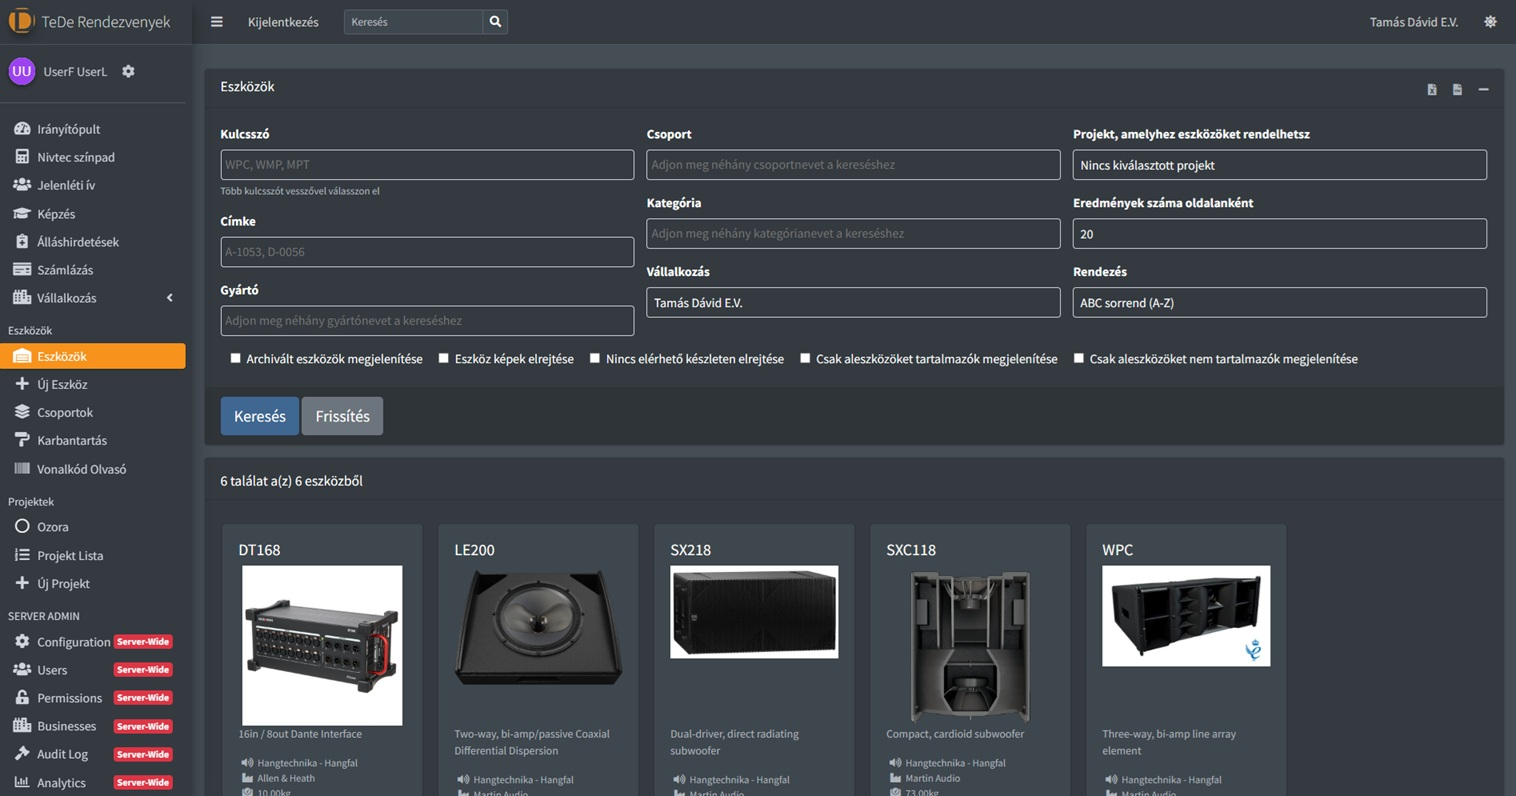
\includegraphics[width=150mm, keepaspectratio]{figures/items.jpg}
    \caption{Eszközök kezelése}
    \label{fig:items}
\end{figure}
%----------------------------------------------------------------------------
\subsection{Projektek kezelése}
%----------------------------------------------------------------------------

A rendszer egyik legfontosabb modulja a \textbf{Projektek kezelése}, amely a vállalkozás teljes operatív működését átfogja.  
Ebben a nézetben a felhasználó részletesen konfigurálhatja és nyomon követheti az egyes eseményekhez, rendezvényekhez vagy megrendelésekhez tartozó projekteket.  
A cél, hogy minden információ, az ügyféltől kezdve az eszközökön és helyszíneken át egészen a csapatbeosztásig, egy központi felületen legyen kezelhető.

A projekt adatlapja több logikai szekcióra tagolódik:

\begin{itemize}
    \item \textbf{Ügyfélkezelés:} a projekthez tartozó ügyféladatokat jeleníti meg, illetve új ügyfél is létrehozható közvetlenül innen.  
    Ez leegyszerűsíti a megrendelések adminisztrációját és a CRM-folyamatok integrációját.

    \item \textbf{Projektmenedzser és felelősök:} minden projekthez hozzárendelhető egy vagy több felelős személy, 
    akik a feladatok koordinálásáért és a végrehajtás felügyeletéért felelősek.  
    A rendszer automatikus értesítéseket küld, ha egy új projektet hoznak létre vagy módosítanak.

    \item \textbf{Helyszínkezelés:} a rendezvény vagy telepítés pontos helyszínét tartalmazza.  
    Az adatbázis képes korábbi helyszínek újrafelhasználására, így a gyakran ismétlődő helyszínek (pl. fesztiválok, partnerrendezvények) gyorsan kiválaszthatók.

    \item \textbf{Logisztikai kalkuláció:} a rendszer automatikusan kiszámítja a raktártól való távolságot, az utazási időt, az üzemanyag-felhasználást és a várható utazási költséget.  
    Ez a funkció különösen fontos a terepi projektek (például rendezvényhelyszínek) előkészítése során, 
    mivel a logisztikai tervezés a költségvetés egyik kritikusabb eleme.

    \item \textbf{Erőforrás-hozzárendelés:} a projektfelülethez közvetlenül csatolhatók eszközök, járművek és utánfutók.  
    A rendszer automatikusan figyelmeztet, ha egy eszköz már másik projekthez van rendelve, vagy ha a projekt inaktív, így elkerülhetők az ütközések és a duplikációk.

    \item \textbf{Eseményidőtartam és ütemezés:} a projekt időtartamát kezdő- és záródátum alapján rögzíti a rendszer, 
    amely később összekapcsolódik a naptármodullal.  
    A felhasználók így a teljes munkafolyamatot, az előkészítéstől az építési napig, kronológiai sorrendben követhetik.
\end{itemize}
%----------------------------------------------------------------------------
\begin{figure}[H]
    \centering
    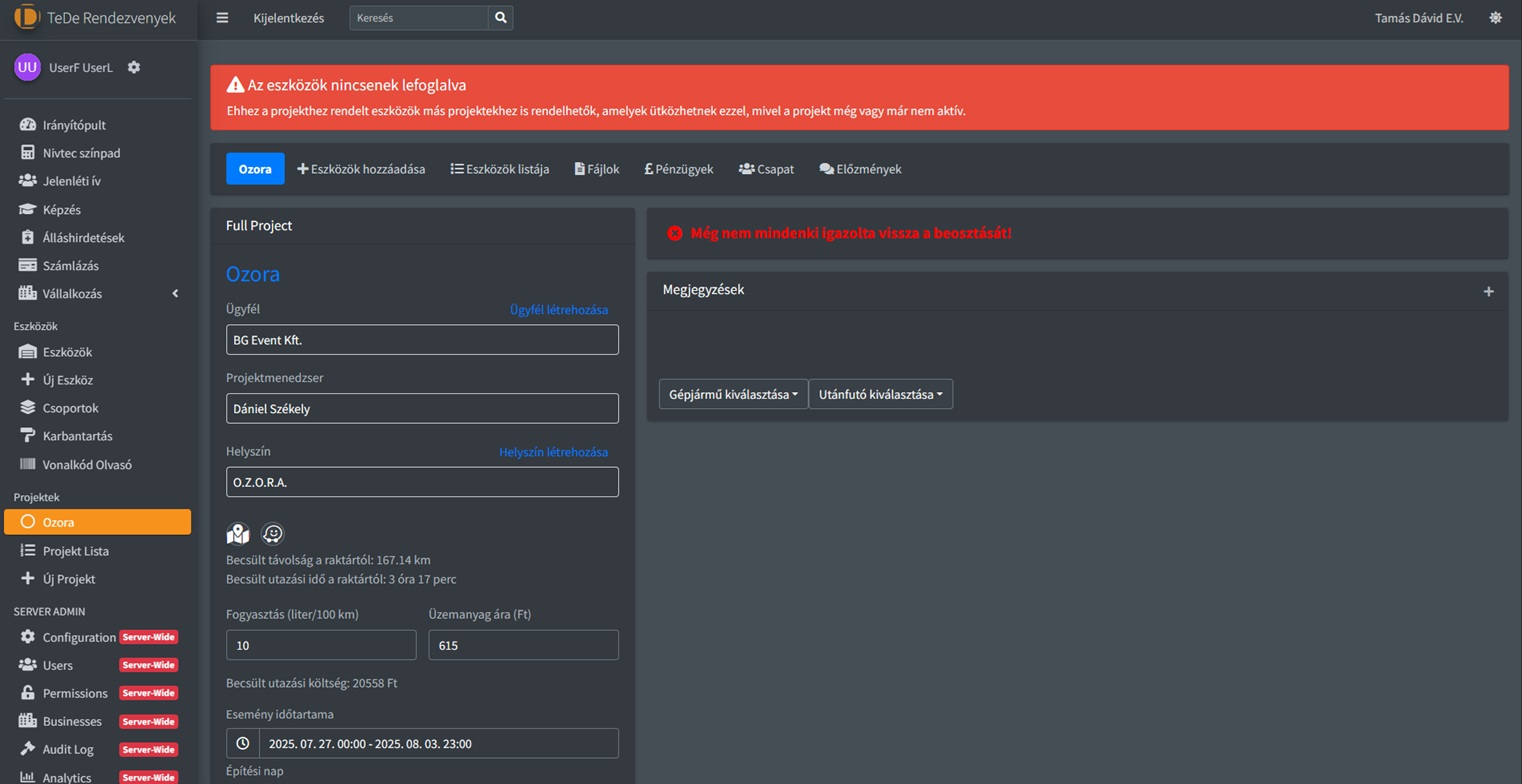
\includegraphics[width=150mm, keepaspectratio]{figures/project.jpg}
    \caption{Projekt részletes adatlap amit az adminok és menedzserek látnak}
    \label{fig:project}
\end{figure}
%----------------------------------------------------------------------------
A projektekhez további funkciók is társulnak, például fájlkezelés (dokumentumok, szerződések, műszaki rajzok feltöltése), pénzügyi modul (költségvetés és elszámolás), 
valamint \textbf{csapatkezelés}, amelyben a rendszer minden résztvevőt listáz és státuszukat (jóváhagyott / függő) megjeleníti.  
Ezáltal a projektmenedzser azonnal látja, ha valaki még nem erősítette meg a beosztását, ezt vizuálisan is jelzi a felület figyelmeztető sávja.

A \textbf{Projektek kezelése} modul így nem csupán adminisztrációs célokat szolgál, hanem valódi menedzsmenteszközzé válik, 
amely integrálja a logisztikai, humán és technikai folyamatokat.  
Ezzel biztosítja, hogy minden esemény előkészítése és lebonyolítása transzparensen, ellenőrzötten és hatékonyan történjen.

A rendszer minden egyes módosítást naplóz, így a projekt életciklusa teljes egészében visszakövethető, ki mikor és milyen változtatást hajtott végre.  
Ez különösen fontos a későbbi auditok és elemzések szempontjából, valamint amennyiben vitás helyzetek merülnének fel a projekt végrehajtása során,
hiszen minden lépés dokumentált és ellenőrizhető marad.
%----------------------------------------------------------------------------
\begin{figure}[H]
    \centering
    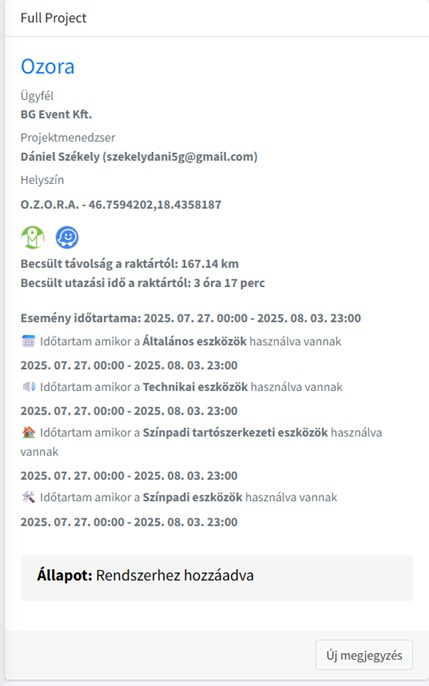
\includegraphics[width=70mm, keepaspectratio]{figures/project_card.jpg}
    \caption{Projekt kompakt adatlap amit a munkavállalók látnak}
    \label{fig:project_card}
\end{figure}
%----------------------------------------------------------------------------
\subsection{GitHub és Reverse Proxy}
%----------------------------------------------------------------------------

A verziókezelés és a biztonságos hálózati hozzáférés is kiemelt szerepet kapott a projekt során.  
A projekt forráskódja a \textbf{GitHub} platformon található, amely lehetővé teszi a verziók követését, a biztonsági mentések készítését és a folyamatos fejlesztést.  
A GitHub használata növeli a fejlesztési folyamat átláthatóságát, támogatja a csapatmunkát, és biztosítja a kód minőségének megőrzését.

A fejlesztés egy főágon (\texttt{main branch}) zajlik, ehhez a lokális környezetből \texttt{git push/pull} műveletekkel történik a szinkronizálás.  
Minden új funkció fejlesztése külön fejlesztői ágon (\texttt{feature branch}) történik, ezáltal a stabil főverzióba csak tesztelt és hibamentes kód kerülhet.  
A commit-ok egységes elnevezési sémát követnek (pl. \texttt{feat:}, \texttt{fix:}, \texttt{refactor:}), ami megkönnyíti a változások visszakövetését és a hibakeresést.  
A verziókezelés így nem csupán biztonsági, hanem projektmenedzsment-eszközként is működik.

A fejlesztési környezet a \textbf{Docker Compose} infrastruktúrán alapul, amely biztosítja a konténerek gyors indítását, újratelepítését és frissítését.  
A rendszer több szolgáltatásból áll — például webalkalmazás, adatbázis és proxy réteg — amelyek egymással biztonságosan kommunikálnak a konténerhálón belül.  
A külső hálózat felé a kapcsolatot egy \textbf{Reverse Proxy} réteg biztosítja, amely a beérkező HTTP(S) kéréseket a megfelelő szolgáltatáshoz irányítja.

A reverse proxy réteg \textbf{NGINX} alapokon működik, amely:
\begin{itemize}
    \item biztosítja a HTTPS titkosítást és a tanúsítványkezelést (\texttt{Let's Encrypt});
    \item lehetővé teszi az aldomének és portok dinamikus irányítását;
    \item csökkenti a külső támadások kockázatát az alkalmazásrétegek elszigetelésével;
    \item elősegíti a terheléselosztást, ezáltal növeli a rendszer válaszképességét és stabilitását.
\end{itemize}

A proxy réteg nemcsak hálózati védelmet nyújt, hanem támogatja a fejlesztés és üzemeltetés szétválasztását is.  
A GitHub repository tartalmazza a \texttt{docker-compose.yml} és \texttt{nginx.conf} fájlokat, amelyek lehetővé teszik a rendszer gyors telepítését bármely környezetben — fejlesztői, teszt vagy éles szerveren — egyetlen parancs segítségével.

Ez az architektúra a modern \textbf{DevOps-elvek} alapján működik, ahol a fejlesztés, verziókezelés, biztonság és üzemeltetés integrált egységet alkot.  
A GitHub–Docker–NGINX kombináció garantálja a kód stabilitását, az infrastruktúra rugalmasságát és az adatbiztonságot, ami alapvető követelmény egy vállalati szintű rendszer esetében.

%----------------------------------------------------------------------------
\begin{figure}[H]
    \centering
    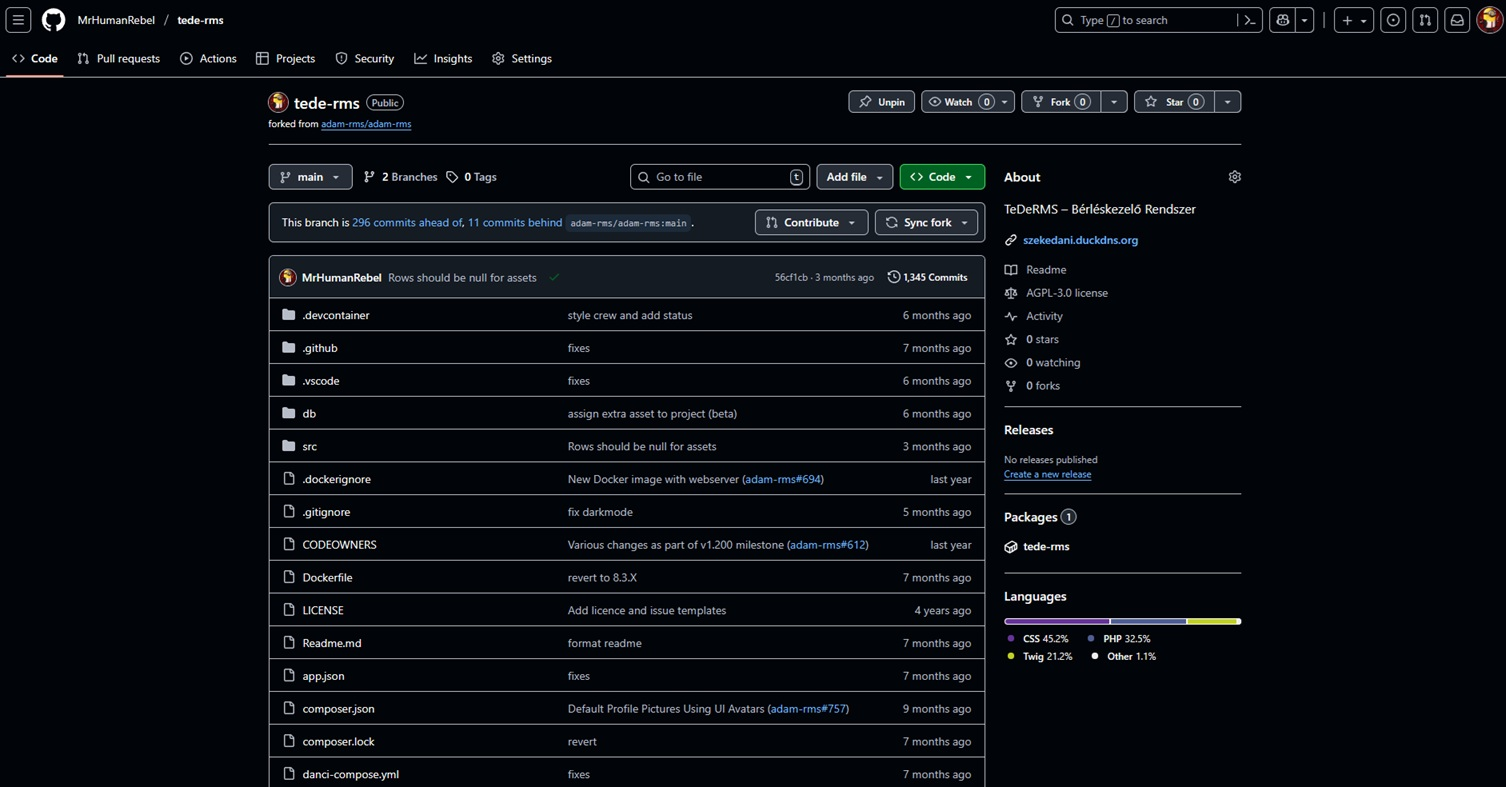
\includegraphics[width=150mm, keepaspectratio]{figures/github.jpg}
    \caption{GitHub repository}
    \label{fig:github}
\end{figure}
%----------------------------------------------------------------------------
%----------------------------------------------------------------------------
\subsection{Kód részletek}
%----------------------------------------------------------------------------
\begin{figure}[H]
    \centering
    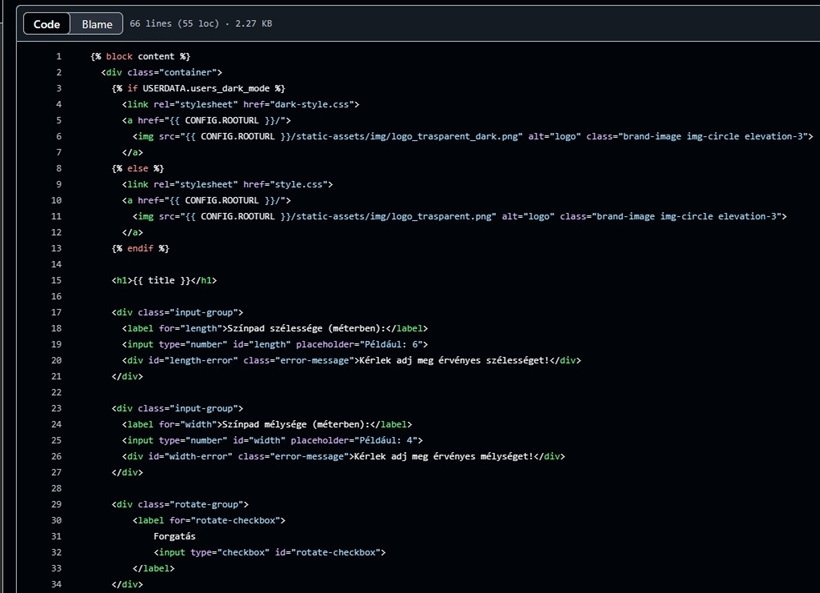
\includegraphics[width=100mm, keepaspectratio]{figures/code_example_nivtec.jpg}
    \caption{Kód részlet - Nivtec kalkulátor integráció}
    \label{fig:code_example_nivtec}
\end{figure}
%----------------------------------------------------------------------------
\begin{figure}[H]
    \centering
    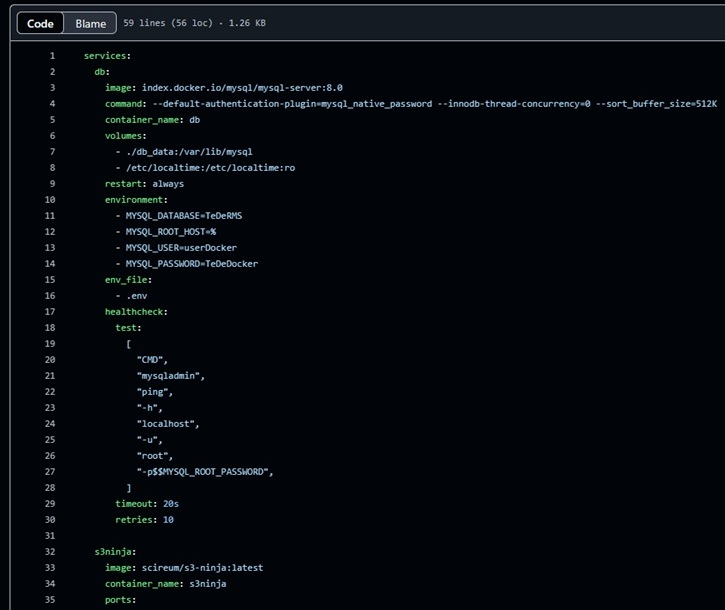
\includegraphics
    [width=100mm, keepaspectratio]{figures/docker_compose.jpg}
    \caption{Kód részlet - Docker Compose fájl}
    \label{fig:docker_compose}
\end{figure}
%----------------------------------------------------------------------------